%%%%%%%%%%%%%%%%%%%%%%%%%%%%%%%%%%%%%%%%%%%%%%%%%%%
%% LaTeX book template                           %%
%% Author:  Amber Jain (http://amberj.devio.us/) %%
%% License: ISC license                          %%
%%%%%%%%%%%%%%%%%%%%%%%%%%%%%%%%%%%%%%%%%%%%%%%%%%%

\documentclass[letterpaper,11pt]{book}
\usepackage[T1]{fontenc}
\usepackage[utf8]{inputenc}
\usepackage{url}
\usepackage{listings}
\usepackage{amsmath}
\usepackage{lmodern}
\usepackage{color}
%%%%%%%%%%%%%%%%%%%%%%%%%%%%%%%%%%%%%%%%%%%%%%%%%%%%%%%%%
% Source: http://en.wikibooks.org/wiki/LaTeX/Hyperlinks %
%%%%%%%%%%%%%%%%%%%%%%%%%%%%%%%%%%%%%%%%%%%%%%%%%%%%%%%%%
\usepackage{hyperref}
\usepackage{graphicx}
\usepackage[english]{babel}
\usepackage{epstopdf}
\usepackage{tikz}
%%%%%%%%%%%%%%%%%%%%%%%%%%%%%%%%%%%%%%%%%%%%%%%%%%%%%%%%%%%%%%%%%%%%%%%%%%%%%%%%
% 'dedication' environment: To add a dedication paragraph at the start of book %
% Source: http://www.tug.org/pipermail/texhax/2010-June/015184.html            %
%%%%%%%%%%%%%%%%%%%%%%%%%%%%%%%%%%%%%%%%%%%%%%%%%%%%%%%%%%%%%%%%%%%%%%%%%%%%%%%%
%\newenvironment{dedication}
%{
%   \cleardoublepage
%   \thispagestyle{empty}
%   \vspace*{\stretch{1}}
%   \hfill\begin{minipage}[t]{0.66\textwidth}
%   \raggedright
%}
%{
%   \end{minipage}
%   \vspace*{\stretch{3}}
%   \clearpage
%}

%%%%%%%%%%%%%%%%%%%%%%%%%%%%%%%%%%%%%%%%%%%%%%%%
% Chapter quote at the start of chapter        %
% Source: http://tex.stackexchange.com/a/53380 %
%%%%%%%%%%%%%%%%%%%%%%%%%%%%%%%%%%%%%%%%%%%%%%%%
%\makeatletter
%\renewcommand{\@chapapp}{}% Not necessary...
%\newenvironment{chapquote}[2][2em]
%  {\setlength{\@tempdima}{#1}%
%   \def\chapquote@author{#2}%
%   \parshape 1 \@tempdima \dimexpr\textwidth-2\@tempdima\relax%
%   \itshape}
%  {\par\normalfont\hfill--\ \chapquote@author\hspace*{\@tempdima}\par\bigskip}
%\makeatother

%%%%%%%%%%%%%%%%%%%%%%%%%%%%%%%%%%%%%%%%%%%%%%%%%%%
% First page of book which contains 'stuff' like: %
%  - Book title, subtitle                         %
%  - Book author name                             %
%%%%%%%%%%%%%%%%%%%%%%%%%%%%%%%%%%%%%%%%%%%%%%%%%%%

% Book's title and subtitle
\title{\huge \textbf{Heat and Mass Transfer in Practice}  \large \textbf{Using Mathematica}. \footnote{This is tutorial for ME 8381.} }
% Author
\author{\textsc{John C. Bischof} \footnote{Professor in Mechanical Engineering of University of Minnesota.}}
%\thanks{\url{www.example.com}}}


\begin{document}

%remove the red rectaugular around the reference.
\hypersetup{pdfborder=0 0 0}
\frontmatter
\maketitle

%%%%%%%%%%%%%%%%%%%%%%%%%%%%%%%%%%%%%%%%%%%%%%%%%%%%%%%%%%%%%%%
% Add a dedication paragraph to dedicate your book to someone %
%%%%%%%%%%%%%%%%%%%%%%%%%%%%%%%%%%%%%%%%%%%%%%%%%%%%%%%%%%%%%%%
%\begin{dedication}
%Dedicated to Calvin and Hobbes.
%\end{dedication}

%%%%%%%%%%%%%%%%%%%%%%%%%%%%%%%%%%%%%%%%%%%%%%%%%%%%%%%%%%%%%%%%%%%%%%%%
% Auto-generated table of contents, list of figures and list of tables %
%%%%%%%%%%%%%%%%%%%%%%%%%%%%%%%%%%%%%%%%%%%%%%%%%%%%%%%%%%%%%%%%%%%%%%%%
\tableofcontents
%\listoffigures
%\listoftables

\mainmatter

%%%%%%%%%%%
% Preface %
%%%%%%%%%%%
%\chapter*{Preface} %will note have index 1, 2, etc.,
\chapter{Introduction to Mathematica}
Mathematica, developed by Wolfram Research\footnote{Wolfram Research is a private company makes computation software}, is a computational software program used in many scientfic, engineering, mathematical and computing fields, based on symbolic mathematics\cite{website:wiki-mathematica}. The programming language using in Mathematica is called Wolfram Language.

\section{Overview}
\subsection{Installation}
Students with a CSE Labs account could download and use \emph{Mathematica} free of charge from \href{https://wwws.cs.umn.edu/download_software/mathematica}{\textcolor{blue} {Mathematica download page}}\footnote{\url{https://wwws.cs.umn.edu/download_software/mathematica}}. By following the instructions from that page, you could install \emph{Mathematica} on Windows, Mac or Linux. 

\begin{figure}[h!]
  \centering
    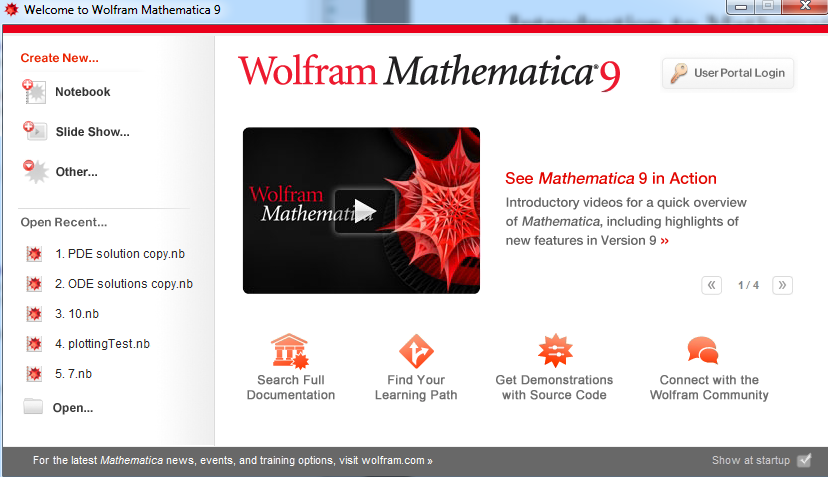
\includegraphics[scale=0.4]{figures/mathematica}
  \caption{Initialization interface of Mathematica}
  \label{fig:mathematica}
\end{figure}

\section{Tutorial}
There are many online tutorials that could help you learning \emph{Wolfram Language} and \emph{Mathematica}. You could find detailed tutorial at \href{http://reference.wolfram.com/language/?source=nav}{\color{blue} Wolfram Language \string& System Documentation Center}\footnote{\url{http://reference.wolfram.com/language/?source=nav}}. Those topics include:
\begin{itemize}
\item Core Language \string& Structure
\item Symbolic \string& Numeric Computation
\item Data Manipulation \string& Analysis
\item Visualization \string& Graphics
\item Images
\item ...
\end{itemize}

There are also many free video courses for educators and researchers which can be found at \href{http://www.wolfram.com/training/courses/edu001.html}{\color{blue} Mathematica for Teaching and Education.}\footnote{\url{http://www.wolfram.com/training/courses/edu001.html}} and
\href{http://www.wolfram.com/training/courses/edu002.html}{\color{blue} Mathematica for University Research}\footnote{\url{http://www.wolfram.com/training/courses/edu002.html}}. In the following section, we will look through some basics of \emph{Wolfram Language}.

\section{Basics}
\subsection{Simple Calculations}
In this section, we will see some examples on some basic arithmetic operations. The Wolfram Language is case sensitive. So
we should use \textbf{Sin} rather than \textbf{sin} to represent
a sinusoidal function.
\\~\\
\textbf{n = 3 + 6}\\
$9$
\\~\\
\textbf{n = 2 + 7 - 8/6}\\
$\frac{23}{3}$
\\~\\
\textbf{Sin[Pi/6]}\\
$\frac{1}{2}$
\\~\\
\textbf{n = Sin[30 Degree]}\\
$\frac{1}{2}$
\\~\\
\textbf{N [Sin[Pi/6]]}\\
$0.5$

\subsection{Matrix Operations}
Vectors and matrices in the Wolfram Language are simply represented by lists and by lists of lists, respectively.
Some basic matrix operations are as shown in Table~\ref{table:matrixOps}.
~\\\\
Expressions of a $3\times3$ matrix:\\
\textbf{m=\{\{-9,19,3\},\{-3,7,1\},\{-7,17,2\}\}}\\
\{\{-9, 19, 3\}, \{-3, 7, 1\}, \{-7, 17, 2\}\}

~\\
Transposing matrix \textbf{m}:\\
\textbf{Transpose[m]}\\
\{\{-9, -3, -7\}, \{19, 7, 17\}, \{3, 1, 2\}\}

~\\
Expressing \textbf{m} in matrix form\textbf{m}:\\
\textbf{MatrixForm[m]}\\
$\left(
\begin{array}{ccc}
 -9 & 19 & 4 \\
 -3 & 7 & 1 \\
 -7 & 17 & 2 \\
\end{array}
\right)$
\\~\\
Inversing matrix \textbf{m}:\\
\textbf{Inverse[m]}\\
$
\left(
\begin{array}{ccc}
 -\frac{3}{2} & \frac{13}{2} & -1 \\
 -\frac{1}{2} & \frac{3}{2} & 0 \\
 -1 & 10 & -3 \\
\end{array}
\right)
$

\begin{table}[h!]
\caption{Basic matrix operations} % title of Table
\centering % used for centering table
\begin{tabular}{c c}
\hline %inserts double horizontal lines
Function & Purpose\\
%heading
\hline % inserts single horizontal line
Transpose[m] & Transpose $m^T$ \\
ConjugateTranspose[m] & Conjugate transpose $m^*$ (Hermitian conjugate) \\
Inverse[m] & Matrix inverse\\
Det[m] & Determinant\\
Tr[m] & Trace\\
MatrixRank[m] & Rank of matrix\\
[1ex] % [1ex] adds vertical space
\hline %inserts single line
\end{tabular}
\label{table:matrixOps} % is used to refer this table in the text
\end{table}

\subsection{Plotting}
The Wolfram Language has many ways to plot functions and data by using function \textbf{Plot}. And it has many options on what the scales should be, how the axes should be draw and so on. In this section, we will see some basic examples on data plotting.
\textbf{Plot[Sin[x], {x, 0, 10}]} gives result shown in Figure \ref{fig:sin}. \textbf{Plot3D[Sin[x]Cos[y], \{x, 0, 5\}, \{y, 1, 10\}]} produces result shown in Figure \ref{fig:sin3D}.\\
\textbf{Plot[Sin[x\string^2],\{x,0,3\},AxesLabel->\{"x value",Sin[x\string^2]\},GridLines->Automatic]} adds label and grid line to the plotting shown in Figure \ref{fig:sinLabel}.
%2\string^3 gives 2^3

\begin{figure}[h!]
  \centering
    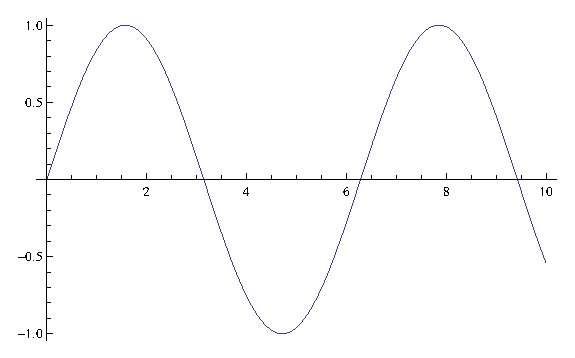
\includegraphics[scale=1]{figures/sin}
  \caption{Plot of $y=sin(x)$}
  \label{fig:sin}
\end{figure}

\begin{figure}[h!]
  \centering
    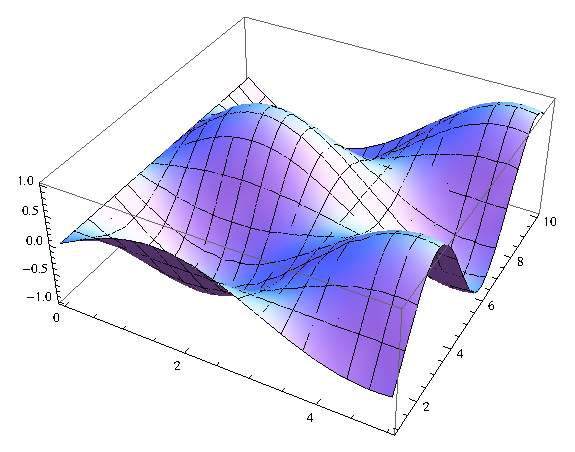
\includegraphics[scale=1]{figures/sin3D}
  \caption{Plot of $z=sin(x)cos(y)$}
  \label{fig:sin3D}
\end{figure}

\begin{figure}[h!]
  \centering
    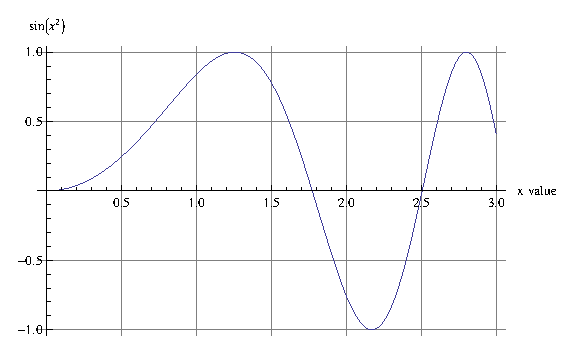
\includegraphics[scale=1]{figures/sinLabel}
  \caption{Plot of $y=sin(x^2)$ with label and axis description}
  \label{fig:sinLabel}
\end{figure}

\subsection{Solving Differential Equation}
Differential equations have three basic types of equations including:
\begin{itemize}
\item \emph{Ordinary Differential Equations} (ODEs), in which there is a single independent variable \textit{t} and one or more dependent variables $x_i(t)$.
\item \emph{Partial Differential Equations} (PDEs), in which there are two or more independent variables and one dependent variable.
\item \emph{Differential-Algebraic Equations} {DAEs}, in which some members of the system are differential equations and the others are purely algebraic, having no derivatives in them.
\end{itemize}

The function \emph{DSolve} gives symbolic solutions to the differential equations while function \emph{NDSolve} generates a general numerical differential equation solver. \emph{DSolve} is powerful in solving ODEs and most first-order PDEs as well as a limited number of the second-order PDEs. For DAEs, it is difficult to find the exact solutions, but \emph{DSolve} can solve many examples of such systems that occur in application.

\subsubsection{Example of solving ODE:}
%setting
\lstset{
language=Mathematica,
basicstyle=\small\sffamily,
%numbers=left,
%numberstyle=\tiny,
frame=tb,
columns=fullflexible,
showstringspaces=false,
mathescape=true
}

%insert mathematica code
\begin{lstlisting}[caption=ODE solution,
  label=code:ode,
  float=t]
eqns = Join[
{x'[t]== -x[t], y'[t]== x[t] - y[t], 
z'[t]== y[t],
x[0]==100,y[0]==0, z[0]==0},
{x,y,z}, {t,10}];
sol = NDSolve[
{x'[t]== -x[t], y'[t]== x[t] - 10y[t], 
z'[t]== 10y[t],
x[0]==100, y[0]==0, z[0]==0},
{x,y,z}, {t,100}];
Plot[
Evaluate[{x[t],y[t],z[t]} /. sol], 
{t,0,10}, 
PlotLegends->Placed[{"x[t]", "y[t]", "z[t]"} , {Right, Bottom}]]
\end{lstlisting}

\begin{figure}[h!]
  \centering
    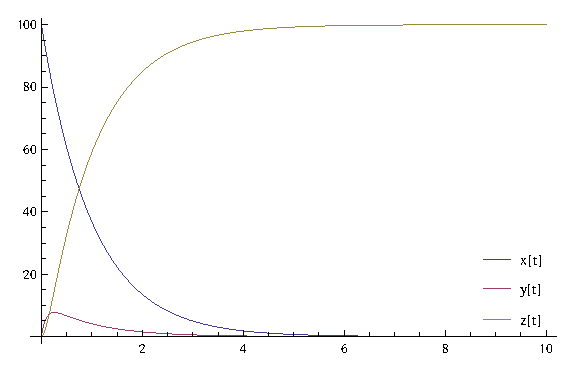
\includegraphics[scale=1]{figures/ODE}
  \caption{Plot of ODE solution}
  \label{fig:ODE}
\end{figure}

\subsubsection{Example of solving PDE:}








%%%%%%%%%%%%%%%%
% NEW CHAPTER! %
%%%%%%%%%%%%%%%%
\chapter{Introductory Chapter}

%\begin{chapquote}{Author's name, \textit{Source of this quote}}
%``This is a quote and I don't know who said this.''
%\end{chapquote}

\section{Section heading}
Lorem ipsum dolor sit amet, consectetur adipisicing elit, sed do eiusmod tempor incididunt ut labore et dolore magna aliqua. Ut enim ad minim veniam, quis nostrud exercitation ullamco laboris nisi ut aliquip ex ea commodo consequat. \\ Duis aute irure dolor in reprehenderit in voluptate velit esse cillum dolore eu fugiat nulla pariatur. Excepteur sint occaecat cupidatat non proident, sunt in culpa qui officia deserunt mollit anim id est laborum. \\ Lorem ipsum list:




1. Lorem ipsum dolor sit amet, consectetur adipiscing elit.

2. Duis ac mi magna, a consectetur elit.

3. Curabitur posuere erat \emph{dignissim ligula euismod} ut euismod nisi.

4. Fusce vulputate facilisis neque, et ornare mauris mattis vel.

5. Mauris sit amet nulla mi, vitae rutrum ante.

6. Maecenas quis nulla risus, vel tincidunt ligula.

7. Nullam ac enim neque, non \emph{dapibus} mauris.

8. Integer volutpat leo a orci suscipit eget rhoncus urna eleifend.

\noindent Lorem ipsum dolor sit amet, consectetur adipiscing elit. Duis risus ante, auctor et pulvinar non, posuere ac lacus. Praesent egestas nisi id metus rhoncus ac lobortis sem hendrerit. Etiam et sapien eget lectus interdum posuere sit amet ac urna\footnote{Lorem ipsum dolor sit amet, consectetur adipiscing elit. Duis risus ante, auctor et pulvinar non, posuere ac lacus.}:

\subsection{Lorem ipsum dolor sit amet, consectetur adipiscing elit.}
Lorem ipsum dolor sit amet, consectetur adipiscing elit. Duis risus ante, auctor et pulvinar non, posuere ac lacus. Praesent egestas nisi id metus rhoncus ac lobortis sem hendrerit. Etiam et sapien eget lectus interdum posuere sit amet ac urna. Aliquam pellentesque imperdiet erat, eget consectetur felis malesuada quis. Pellentesque sollicitudin, odio sed dapibus eleifend, magna sem luctus turpis, id aliquam felis dolor eu diam. Etiam ullamcorper, nunc a accumsan adipiscing, turpis odio bibendum erat, id convallis magna eros nec metus. Sed vel ligula justo, sit amet vestibulum dolor. Sed vitae augue sit amet magna ullamcorper suscipit. Quisque dictum ipsum a sapien egestas facilisis.

Lorem ipsum dolor sit amet, consectetur adipiscing elit. Duis risus ante, auctor et pulvinar non, posuere ac lacus. Praesent egestas nisi id metus rhoncus ac lobortis sem hendrerit. Etiam et sapien eget lectus interdum posuere sit amet ac urna.

\subsection{Lorem ipsum dolor sit amet, consectetur adipiscing.}
Lorem ipsum dolor sit amet, consectetur adipiscing elit. Duis risus ante, auctor et pulvinar non, posuere ac lacus. Praesent egestas nisi id metus rhoncus ac lobortis sem hendrerit. Etiam et sapien eget lectus interdum posuere sit amet ac urna. Aliquam pellentesque imperdiet erat, eget consectetur felis malesuada quis. Pellentesque sollicitudin, odio sed dapibus eleifend, magna sem luctus turpis, id aliquam felis dolor eu diam.

\subsection{Lorem ipsum dolor sit amet}
Lorem ipsum dolor sit amet, consectetur adipiscing elit. Duis risus ante, auctor et pulvinar non, posuere ac lacus. Praesent egestas nisi id metus rhoncus ac lobortis sem hendrerit. Etiam et sapien eget lectus interdum posuere sit amet ac urna. Aliquam pellentesque imperdiet\footnote{\url{www.example.com}} erat, eget consectetur felis malesuada quis. Pellentesque sollicitudin, odio sed dapibus eleifend, magna sem luctus turpis, id aliquam felis dolor eu diam. Etiam ullamcorper, nunc a accumsan adipiscing, turpis odio bibendum erat, id convallis magna eros nec metus. Sed vel ligula justo, sit amet vestibulum dolor. Sed vitae augue sit amet magna ullamcorper suscipit. Quisque dictum ipsum a sapien egestas facilisis.

In hac habitasse platea dictumst. Nullam turpis erat, porttitor ut pretium ac, condimentum sed dui. Praesent arcu elit, tristique sit amet viverra at, auctor quis tortor. Etiam eleifend posuere aliquam. Donec sed mattis sapien. Aenean urna arcu, suscipit at rutrum ac, adipiscing ac felis. Class aptent taciti sociosqu ad litora torquent per conubia nostra, per inceptos himenaeos. Praesent condimentum felis a ipsum ullamcorper semper. Vivamus eu odio sem, dictum luctus nunc. Etiam tincidunt venenatis dolor non pellentesque.

\subsection{Lorem ipsum dolor sit amet, auctor et pulvinar non}
Lorem ipsum dolor sit amet, consectetur adipiscing elit. Duis risus ante, auctor et pulvinar non, posuere ac lacus. Praesent egestas nisi id metus rhoncus ac lobortis sem hendrerit. Etiam et sapien eget lectus interdum posuere sit amet ac urna. Aliquam pellentesque imperdiet erat, eget consectetur felis malesuada quis. Pellentesque sollicitudin, odio sed dapibus eleifend, magna sem luctus turpis, id aliquam felis dolor eu diam. Etiam ullamcorper, nunc a accumsan adipiscing, turpis odio bibendum erat, id convallis magna eros nec metus. Sed vel ligula justo, sit amet vestibulum dolor. Sed vitae augue sit amet magna ullamcorper suscipit. Quisque dictum ipsum a sapien egestas facilisis.

In hac habitasse platea dictumst. Nullam turpis erat, porttitor ut pretium ac, condimentum sed dui. Praesent arcu elit, tristique sit amet viverra at, auctor quis tortor. Etiam eleifend posuere aliquam. Donec sed mattis sapien. Aenean urna arcu, suscipit at rutrum ac, adipiscing ac felis. Class aptent taciti sociosqu ad litora torquent per conubia nostra, per inceptos himenaeos. Praesent condimentum felis a ipsum ullamcorper semper. Vivamus eu odio sem, dictum luctus nunc. Etiam tincidunt venenatis dolor non pellentesque. 


\section{Another section heading}
Lorem ipsum dolor sit amet, consectetur adipisicing elit, sed do eiusmod tempor incididunt ut labore et dolore magna aliqua. Ut enim ad minim veniam, quis nostrud exercitation ullamco laboris nisi ut aliquip ex ea commodo consequat.

%%%%%%%%%%%%%%%%%%%%%%%%%%%%%%%%%%%%%%%%%%%%%%%%%%%%%%%
% Sample table                                        %
% Source: www1.maths.leeds.ac.uk/latex/TableHelp1.pdf %
%%%%%%%%%%%%%%%%%%%%%%%%%%%%%%%%%%%%%%%%%%%%%%%%%%%%%%%
\begin{table}[ht]
\caption{Sample table} % title of Table
\centering % used for centering table
\begin{tabular}{c c c c}
% centered columns (4 columns)
\hline\hline %inserts double horizontal lines
S. No. & Column\#1 & Column\#2 & Column\#3 \\ [0.5ex]
% inserts table
%heading
\hline % inserts single horizontal line
1 & 50 & 837 & 970 \\
2 & 47 & 877 & 230 \\
3 & 31 & 25 & 415 \\
4 & 35 & 144 & 2356 \\
5 & 45 & 300 & 556 \\ [1ex] % [1ex] adds vertical space
\hline %inserts single line
\end{tabular}
\label{table:nonlin} % is used to refer this table in the text
\end{table}

Duis aute irure dolor in reprehenderit in voluptate velit esse cillum dolore eu fugiat nulla pariatur. Excepteur sint occaecat cupidatat non proident, sunt in culpa qui officia deserunt mollit anim id est laborum. \\ Lorem ipsum list:
\begin{itemize}
\item Mauris sit amet nulla mi, vitae rutrum ante.
\item Maecenas quis nulla risus, vel tincidunt ligula.
\item Nullam ac enim neque, non \emph{dapibus} mauris.
\end{itemize}

\noindent Lorem ipsum dolor sit amet, consectetur adipiscing elit. Duis risus ante, auctor et pulvinar non, posuere ac lacus. Praesent egestas nisi id metus rhoncus ac lobortis sem hendrerit. Etiam et sapien eget lectus interdum posuere sit amet ac urna\footnote{Lorem ipsum dolor sit amet, consectetur adipiscing elit. Duis risus ante, auctor et pulvinar non, posuere ac lacus.}:

\subsection{Lorem ipsum dolor sit amet, consectetur adipiscing elit.}
Lorem ipsum dolor sit amet, consectetur adipiscing elit. Duis risus ante, auctor et pulvinar non, posuere ac lacus. Praesent egestas nisi id metus rhoncus ac lobortis sem hendrerit. Etiam et sapien eget lectus interdum posuere sit amet ac urna. Aliquam pellentesque imperdiet erat, eget consectetur felis malesuada quis. Pellentesque sollicitudin, odio sed dapibus eleifend, magna sem luctus turpis, id aliquam felis dolor eu diam. Etiam ullamcorper, nunc a accumsan adipiscing, turpis odio bibendum erat, id convallis magna eros nec metus. Sed vel ligula justo, sit amet vestibulum dolor. Sed vitae augue sit amet magna ullamcorper suscipit. Quisque dictum ipsum a sapien egestas facilisis. 

\subsection{Lorem ipsum dolor sit amet, consectetur adipiscing}
Lorem ipsum dolor sit amet, consectetur adipiscing elit. Duis risus ante, auctor et pulvinar non, posuere ac lacus. Praesent egestas nisi id metus rhoncus ac lobortis sem hendrerit. Etiam et sapien eget lectus interdum posuere sit amet ac urna. Aliquam pellentesque imperdiet erat, eget consectetur felis malesuada quis. Pellentesque sollicitudin, odio sed dapibus eleifend, magna sem luctus turpis, id aliquam felis dolor eu diam.


%setting
\lstset{
language=Mathematica,
basicstyle=\small\sffamily,
%numbers=left,
%numberstyle=\tiny,
frame=tb,
columns=fullflexible,
showstringspaces=false,
mathescape=true
}

%insert mathematica code
\begin{lstlisting}[caption=Code for constant heat,
  label=a_label,
  float=t]
(* $q_m$: volumetric heat release *)
$q_m$ = 100;
(* k: thermal conductivity *)
k = 0.4;
(* $T_0$: temperature at the position x=0 *)
$T_0 = 37$;
(* Subscript[T, 0]: temperature at the position x=L=0.1 *)
Subscript[T, 1] = 33;
(* wall thickness *)
L = 0.1;
solution1 =  NDSolve[{
   T''[x] + Subscript[q, m] == 0, 
   T[0] == Subscript[T, 0],
   T[0.04] == Subscript[T, 1]},
   T,
   {x, 0, 0.04}];
PS1 = Plot[Evaluate[T[x] /. First[solution1]], {x, 0, 0.1}, PlotRange -> All];
\end{lstlisting}


\bibliographystyle{plain}
\bibliography{bibliography/MathematicaTutorial}

\end{document}










